\documentclass[10pt,a4paper]{article}
\usepackage[utf8]{inputenc}
\usepackage[french]{babel}
\usepackage[T1]{fontenc}
\usepackage{graphicx}
\usepackage{listings}

\usepackage{fancyhdr}
\usepackage{vmargin}
\usepackage{amsmath}

\setlength{\parindent}{0cm}
\setlength{\parskip}{1ex plus 0.5ex minus 0.2ex}
\newcommand{\hsp}{\hspace{20pt}}
\newcommand{\HRule}{\rule{\linewidth}{0.5mm}}

\begin{document}
	\pagestyle{fancy}
	\fancyhf{}
	\rhead{SALEMI Marco, LECOCQ Alexis}
	\lhead{Pi randomness}
	\cfoot{\thepage}
	
	\begin{titlepage}
		\begin{center}
			% Upper part of the page. The '~' is needed because \\
			% only works if a paragraph has started.
			
\includegraphics[scale=1.5]{images/pi.png}~\\[1.5cm]
			
			% Title
			\HRule \\[0.5cm]
			{ \huge \bfseries Pi randomness\\[0.4cm] }
			\HRule \\[1.5cm]
			
			\Large{Rapport de projet de simulation}\\[2cm]
			
			\Large{Année académique 2016-2017}\\[2cm]
			
			% Author and supervisor
			\begin{minipage}{0.4\textwidth}
				\begin{flushleft} \large
					\emph{\textbf{Auteurs :}}\\
					SALEMI Marco\\
					LECOCQ Alexis
				\end{flushleft}
			\end{minipage}
			\begin{minipage}{0.4\textwidth}
				\begin{flushright} \large
					\emph{\textbf{Directeurs :}}\\
					BUYS Alain\\
					-\\
				\end{flushright}
			\end{minipage}
			
			\vfill
			
			% Bottom of the page
			{\large \today}
			
		\end{center}
	\end{titlepage}
	
	\newpage
	\tableofcontents
	
	\newpage
	\section{Introduction}
	Dans le cadre du cours de simulation, nous avons été amenés à réaliser un projet afin de mettre en pratique la théorie vue au cours.
	
	Les objectifs du projet sont :
	\begin{enumerate}
		\item analyser le caractère aléatoire des décimales de pi par des tests vus au cours ;
		\item utiliser ces décimales pour construire un générateur de loi uniforme dans l'intervalle [0, 1[ ;
		\item comparer le générateur du point 2 avec celui utilisé par défaut dans Python.
	\end{enumerate}
	
	Pour ce faire, un fichier nous est fourni. Celui-ci contient les 1 000 000 premières décimales du nombre pi.
	
	Le projet doit être réalisé en python et nous avons opté pour la version 3.

	Nous avons utilisé deux librairies externes :
	\begin{itemize}
		\item \textbf{scipy} : pour l'accès à la table des valeurs de Kolmogorov-Smirnov ;
		\item \textbf{plotly} : pour réaliser les graphiques.
	\end{itemize}
	
	L'installation de ces libraires est très simple à l'aide du gestionnaire de paquets pip3 :
	
	\begin{center}
		\begin{tabular}{|l|}
			\hline \\
			\$ pip3 install scipy plotly\\
			\\
			\hline
		\end{tabular}
	\end{center}
	
	Sur certains systèmes, les droits administrateurs sont requis pour installer des librairies.
	
	\newpage
	\section{Les décimales de $\pi$}
	
	\subsection{Test de $\chi^2$}
	Le premier test consiste à étudier le nombre d'apparitions de chaque décimale. Si la séquence suit une loi uniforme, l'ensemble des décimales apparaissent exactement le même nombre de fois.
	
	
	Résultats du test :
	\begin{figure}[h]
		\centering
		\begin{tabular}{|r|r|r|}
			\hline
			Décimales & Valeur attendue & Valeur observée\\
			\hline
			0 & 100000 & 99959\\
			1 & 100000 & 99758\\
			2 & 100000 & 100026\\
			3 & 100000 & 100229\\
			4 & 100000 & 100230\\
			5 & 100000 & 100359\\
			6 & 100000 & 99548\\
			7 & 100000 & 99800\\
			8 & 100000 & 99985\\
			9 & 100000 & 100106\\
			\hline
		\end{tabular}
		\caption{Tableau des décimales}
	\end{figure}
	
	Graphique :
	\begin{figure}[h]
		\centering
		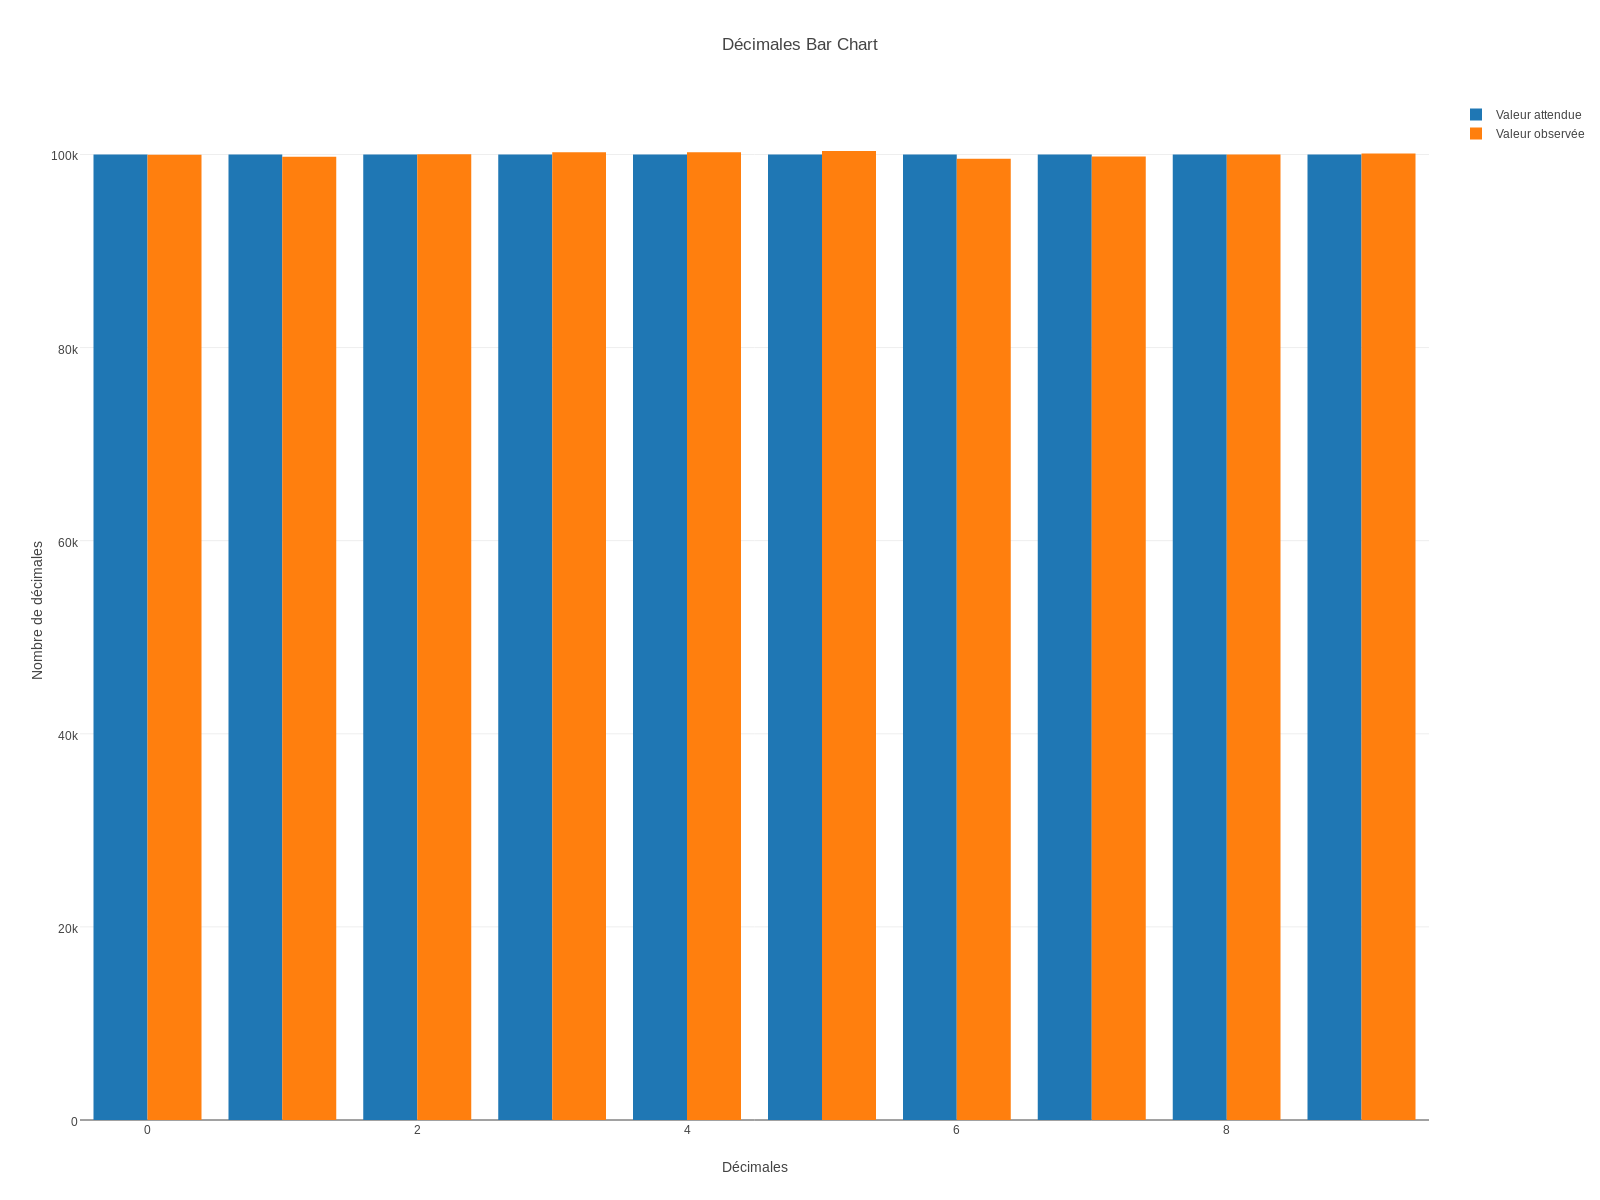
\includegraphics[scale=0.25]{../chart_images/decimales_bar_chart.png}
		\caption{Graphique des décimales}
	\end{figure}
	
	\newpage
	Test de $\chi^2$ :
	\begin{figure}[h]
		\centering
		\begin{tabular}{|r|r|r|r|}
			\hline
			$\alpha$ & Valeur & Limite & Résultat\\
			\hline
			0.001 & 5.509 & 27.877 & réussi\\
			0.01 & 5.509 & 21.666 & réussi\\
			0.05 & 5.509 & 16.919 & réussi\\
			0.1 & 5.509 & 14.684 & réussi\\
			\hline
		\end{tabular}
		\caption{Tableau du $\chi^2$}
	\end{figure}
	
	Comme nous pouvons le voir dans le tableau, le test est réussi pour tous les $\alpha$ choisis.
	
	\newpage
	\subsection{Test du poker}
	
	Le test du poker consiste à considérer une suite de décimales comme une suite de paquets de $l$ décimales. Dans chaque paquet, on compte le nombre de décimales différentes qui le composent. On regroupe ensuite les paquets par le nombre de décimales différentes qui les composent.
	
	Dans le cas où la séquence de décimales suivrait une loi uniforme, la probabilité d'avoir r décimales différentes dans une séquence de longueur l est de :
	\[
		\frac{
			\left\{
				\begin{array}{l}
					l\\
					r\\
				\end{array}
			\right\}
			\prod_{i=10-r+1}^{10}i
		}{10^l}
	\]
	
	où $\left\{
	\begin{array}{l}
	l\\
	r\\
	\end{array}
	\right\}$ est le nombre de Stirling.
	
	 Pour obtenir la valeur théorique, on multiple la probabilité par le nombre total de paquets. On a opté dans ce test pour des paquets de 5 décimales.
	
	Résultats du test :
	\begin{figure}[h]
		\centering
		\begin{tabular}{|r|r|r|}
			\hline
			\# Décimales $\ne$ & Valeur attendue & Valeur observée\\
			\hline
			1 & 20 & 13\\
			2 & 2700 & 2644\\
			3 & 36000 & 36172\\
			4 & 100800 & 100670\\
			5 & 60480 & 60501\\
			\hline
		\end{tabular}
		\caption{Tableau du Poker}
	\end{figure}
	
	\newpage
	Graphique :
	\begin{figure}[h]
		\centering
		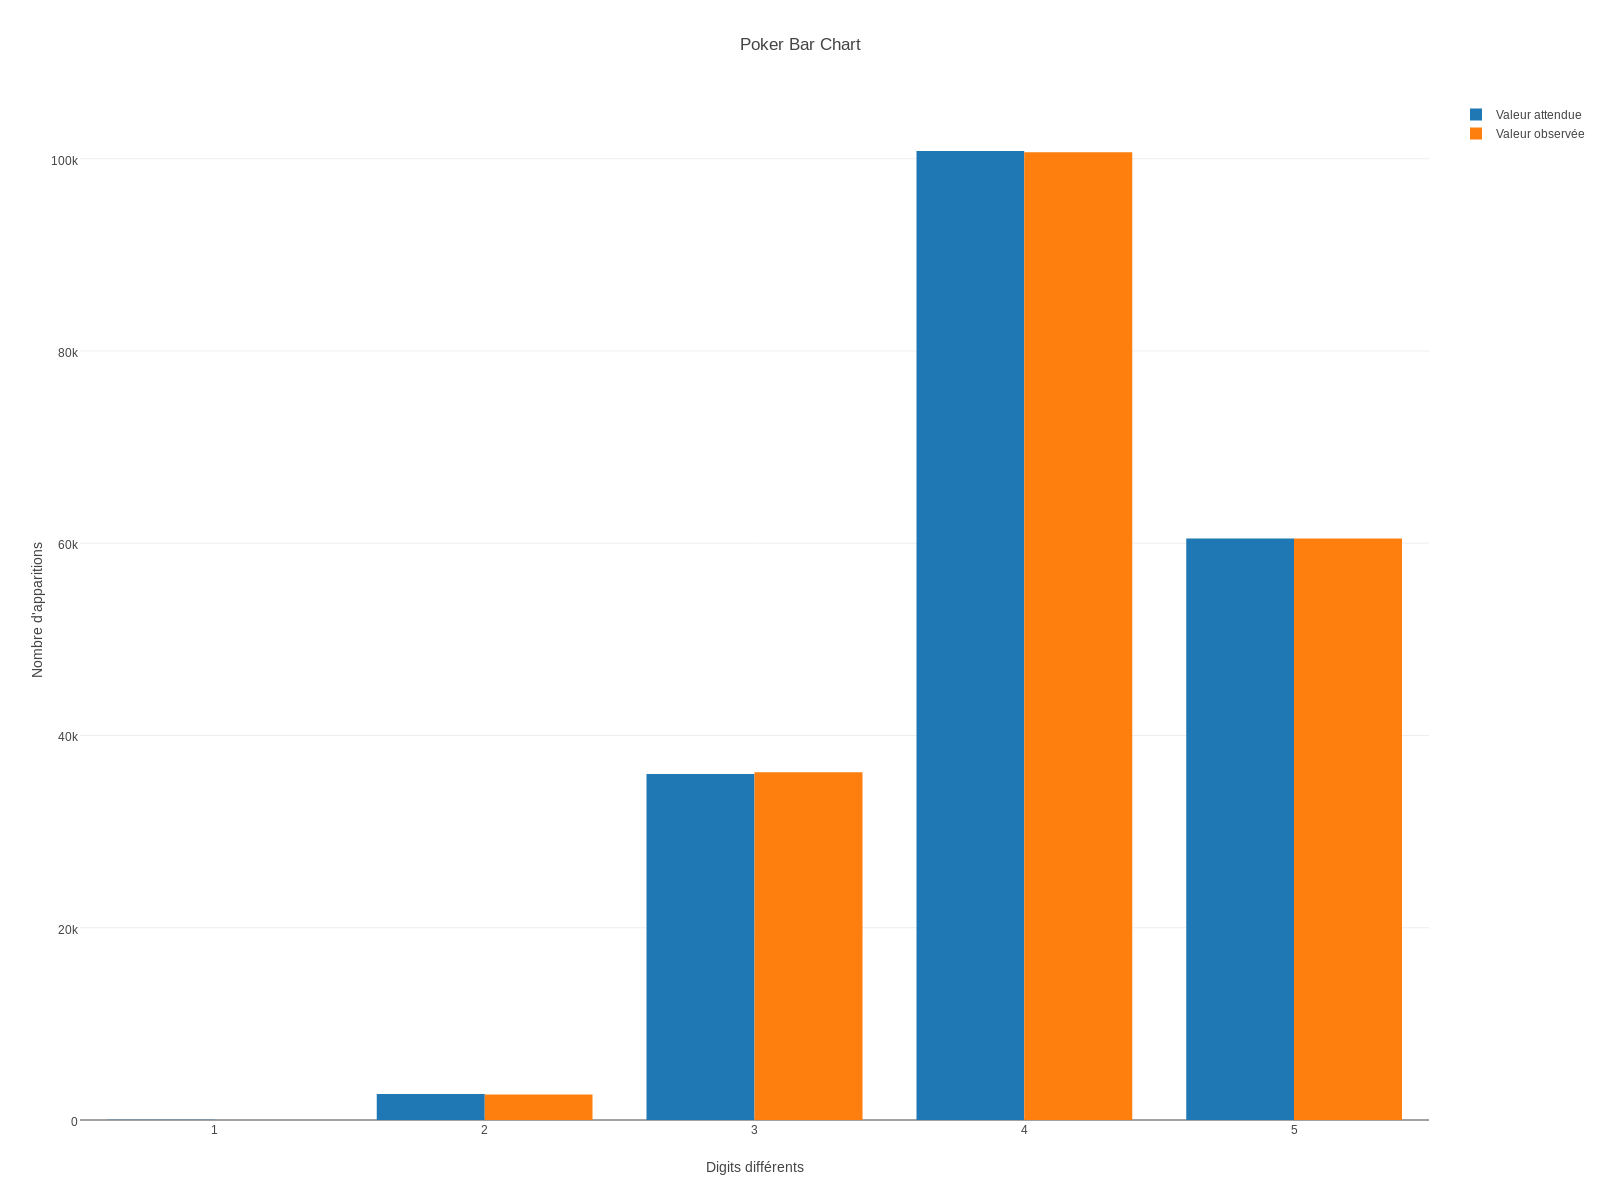
\includegraphics[scale=0.25]{../chart_images/poker_bar_chart.png}
		\caption{Graphique du Poker}
	\end{figure}
	
	Test de $\chi^2$ :
	\begin{figure}[h]
		\centering
		\begin{tabular}{|r|r|r|r|}
			\hline
			$\alpha$ & Valeur & Limite & Résultat\\
			\hline
			0.001 & 4.608 & 18.467 & réussi\\
			0.01 & 4.608 & 13.277 & réussi\\
			0.05 & 4.608 & 9.488 & réussi\\
			0.1 & 4.608 & 7.779 & réussi\\
			\hline
		\end{tabular}
		\caption{Tableau du $\chi^2$}
	\end{figure}
	
	Comme nous pouvons le voir dans le tableau, le test est réussi pour tous les $\alpha$ choisis.
		
\newpage
	
\subsection{Test du collectionneur de coupons}
Le collectionneur de coupons est un test vérifiant la longueur des séquences contenant toutes les décimales. Le fonctionnement est le suivant :  
\begin{itemize}
	\item En fonction du nombre de décimales, nous choisissons une taille maximale à comptabiliser. Les séquences dépassant cette limite seront comptabilisées ensemble à la fin du tableau. Nous avons choisi 85 afin de na pas avoir de classes vides mais de garder un nombre de classes assez élevé.
\item Nous parcourons les différentes décimales de Pi dans l'ordre, en calculant la taille des séquences successives contenant tous les digits (de 0 à 9).
\item Nous tenons compte du nombre de séquences de chaque taille qui a été parcourue.
\end{itemize}

Nous comparons ensuite la taille des séquences observées à la valeur théorique suivant une loi uniforme, et ceci à l'aide d'un $\chi^2$.

Nous calculons la valeur théorique à l'aide de la probabilité $ S_r$ ci-dessous. Celle-ci représente la probabilité qu'une séquence de longueur r contienne toutes les décimales. Ici, d représente le nombre de décimales différentes possibles (10 dans notre cas).

\begin{figure}[h]
		\centering
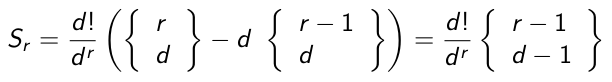
\includegraphics[scale=0.4]{images/formule.png}  
\caption{Probabilité de Coupons}
	\end{figure}

\textbf{Remarque :} $S_r$ sera égal à 0 lorsque r < d. En effet, il est improbable qu'une séquence de longueur inférieure à d contienne d différentes décimales.

La probabilité qu'une séquence soit de longueur supérieure à une certaine limite t (ici 85) est la suivante :

\begin{figure}[h]
		\centering
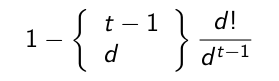
\includegraphics[scale=0.4]{images/formule2.png}  
\caption{Probabilité de Coupons, dernière classe}
	\end{figure}

\newpage

\begin{figure}[h]
\centering
\begin{tabular}{|r|r|r|}
\hline
Tailles de séquences & Valeur attendue & Valeur observée\\
\hline
10 & 12.39706944 & 12\\
11 & 55.78681248 & 62\\
12 & 143.186152032 & 154\\
13 & 276.144721776 & 265\\
14 & 445.677125782 & 496\\
15 & 636.605631934 & 645\\
16 & 832.196551932 & 869\\
17 & 1017.53193425 & 1008\\
18 & 1181.29471772 & 1150\\
19 & 1316.26375399 & 1341\\
20 & 1418.98670105 & 1354\\
21 & 1489.0470501 & 1482\\
22 & 1528.21745078 & 1576\\
23 & 1539.67053158 & 1515\\
24 & 1527.32748565 & 1543\\
25 & 1495.36642995 & 1456\\
26 & 1447.88033297 & 1470\\
27 & 1388.65981367 & 1345\\
28 & 1321.07229861 & 1317\\
29 & 1248.01086229 & 1224\\
30 & 1171.89036844 & 1145\\
\hline
\end{tabular}
\caption{Tableau de Test du CDC : Les décimales de Pi 1}
\end{figure}

\newpage

\begin{figure}[h]
\centering
\begin{tabular}{|r|r|r|}
\hline
Tailles de séquences & Valeur attendue & Valeur observée\\
\hline
31 & 1094.67343335 & 1105\\
32 & 1017.91330149 & 1018\\
33 & 942.804564011 & 968\\
34 & 870.235668768 & 883\\
35 & 800.839427633 & 817\\
36 & 735.039345563 & 772\\
37 & 673.090709825 & 680\\
38 & 615.116112395 & 640\\
39 & 561.135537135 & 522\\
40 & 511.091408294 & 506\\
50 & 190.177745431 & 185\\
60 & 67.624416886 & 69\\
70 & 23.7210160015 & 27\\
71 & 21.3552335886 & 25\\
72 & 19.2247660837 & 27\\
73 & 17.3063345114 & 17\\
74 & 15.5789373362 & 8\\
75 & 14.0236327962 & 12\\
76 & 12.6233409926 & 12\\
77 & 11.3626641589 & 5\\
78 & 10.2277236148 & 13\\
79 & 9.20601199223 & 9\\
80 & 8.28625941323 & 12\\
81 & 7.45831238842 & 8\\
82 & 6.71302429704 & 7\\
83 & 6.04215639528 & 8\\
84 & 5.43828838508 & 4\\
85 & 44.0637637982 & 48\\
\hline
\end{tabular}
\caption{Tableau de Test du CDC : Les décimales de Pi 3}
\end{figure}

\newpage

\begin{figure}[h]
\centering
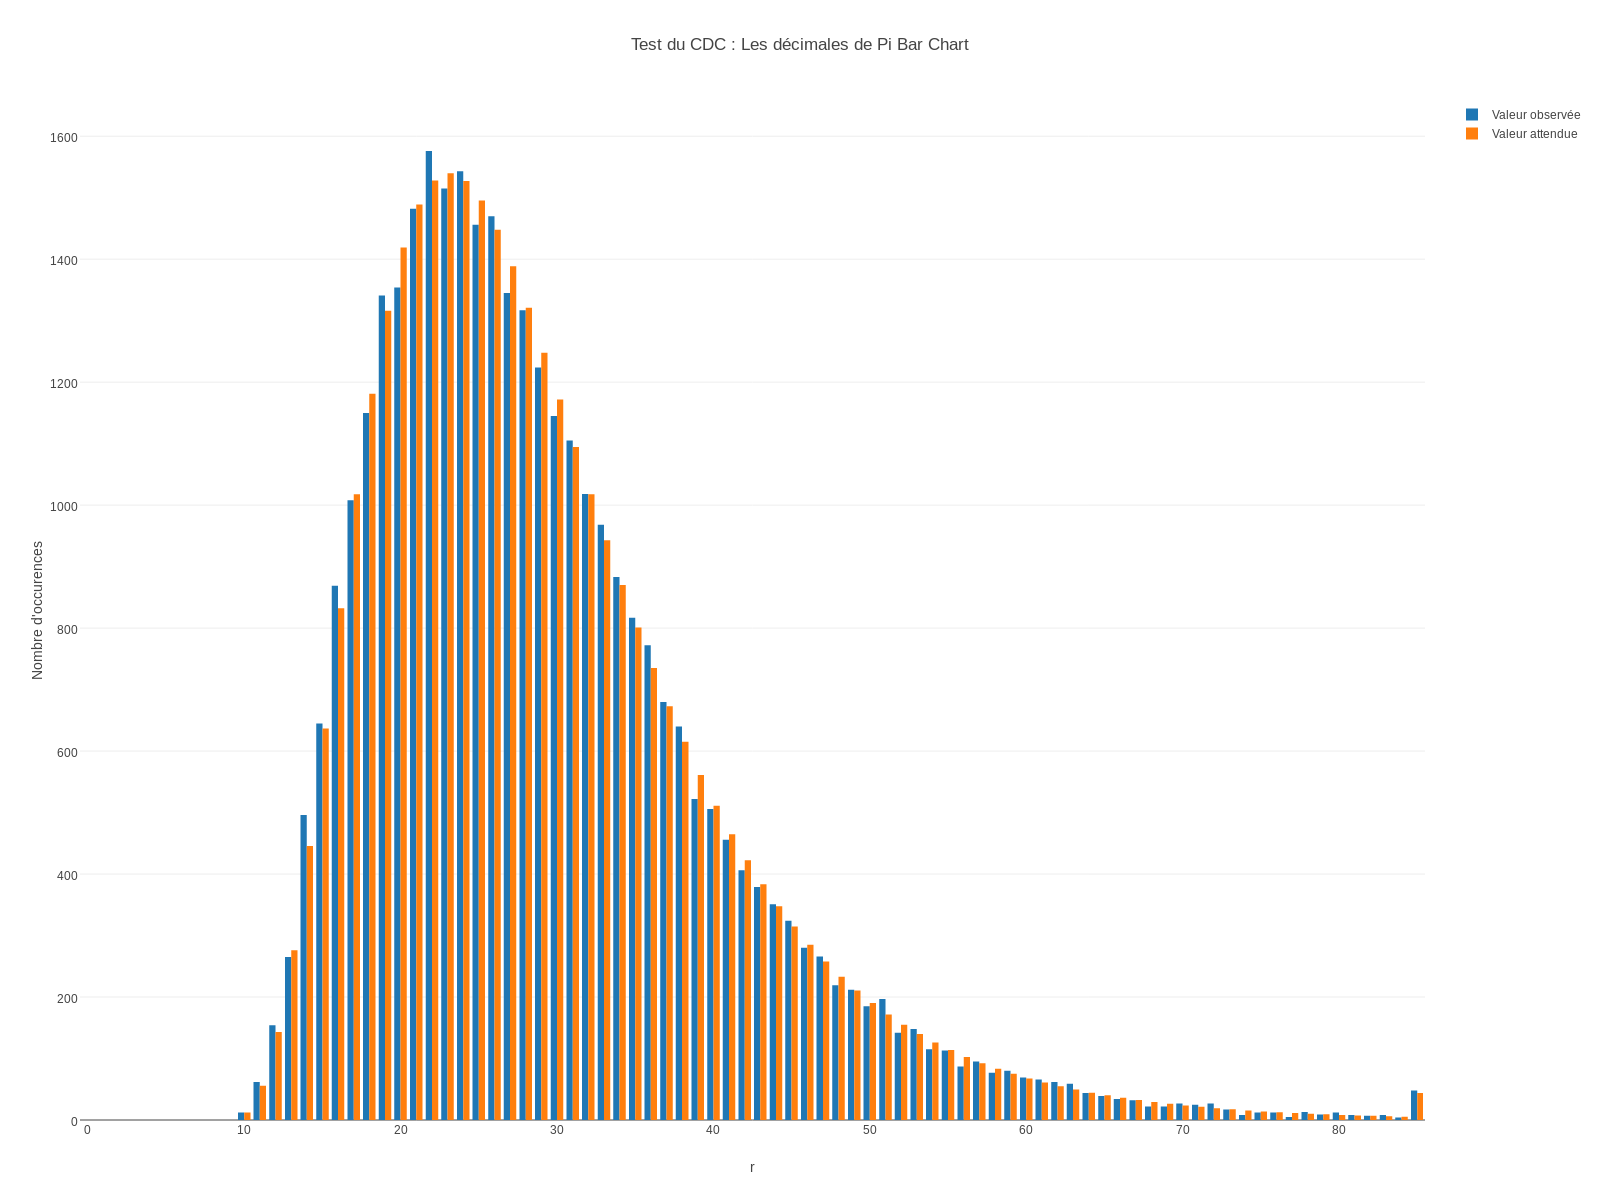
\includegraphics[scale=0.3]{../chart_images/cdc_deci.png}
\caption{Graphique de Test du CDC : Les décimales de Pi}
\end{figure}


\begin{figure}[h]
\centering
\begin{tabular}{|r|r|r|r|}
\hline
$\alpha$ & AValeur & Limite & Résultat\\
\hline
0.001 & 60.226 & 131.041 & réussi\\
0.010 & 60.226 & 118.236 & réussi\\
0.050 & 60.226 & 107.522 & réussi\\
0.100 & 60.226 & 102.079 & réussi\\
\hline
\end{tabular}
\caption{Tableau de $\chi^2$}
\end{figure}


Nous remarquons que les valeurs du tableau sont proches des valeurs théoriques. Ainsi que notre graphique suit la forme d'une gaussienne. 

Ce test confirme donc que les décimales de Pi suivent bien une loi uniforme, car les différents tests de $\chi^2$ sont respectés.

\newpage

\subsection{Interprétation des résultats}
D'après les tests effectués ci-dessus, les décimales de pi suivent bien une loi uniforme.


	\section{Générateur de loi uniforme à partir des décimales de $\pi$}
	Notre générateur est très simple, il suit ces étapes :
	\begin{enumerate}
		\item lecture des $n$ premiers chiffres à l'emplacement actuel comme un nombre ;
		\item division de ce nombre par $10^{n}$ afin d'obtenir un nombre dans l'intervalle $[0, 1[$.
	\end{enumerate}
	Les caractères éventuellement manquants à la fin du fichiers sont lus en début de fichier. Ainsi, le générateur ne s'arrête jamais.
	
	Afin que le générateur ne commence pas toujours la séquence au même emplacement, nous choisissons l'emplacement de départ en fonction d'un timestamp.
	Ce timestamp représente le nombre de millisecondes écoulées depuis le 1er janvier 1970 UTC.
	
	Notre générateur possédant un paramètre $n$, sa période est variable.
	
	\subsection{Choix du paramètre}
	Paramétrer notre générateur soulève une question : quel paramètre utiliser par défaut et pourquoi ?
	
	Choisir un paramètre trop petit réduirait la précision du générateur.
	Par exemple si un seul digit est lu, alors il est évident que notre générateur ne générera que 10 nombres différents.
	Afin d'obtenir la meilleure précision possible, nous nous sommes fixé un minimum de 15 digits.
	Cela correspond à la précision utilisée par Python pour représenter u nombre flottant.
	Augmenter $n$ au-delà de 15 n'améliorerait donc pas la précision.
	
	Par ailleurs, choisir un paramètre qui divise 1000000 réduirait la période.
	Par exemple, si nous choisissons un paramètre de 100, alors il est évident qu'après 10000 générations, nous nous retrouverions au début du fichier.
	Cela réduirait la période à 10000.
	En fait, il convient d'utiliser un nombre qui est premier par rapport à 1000000 pour obtenir la période maximale de 1000000.
	
	Notre premier choix s'est donc porté sur le nombre $n = 17$, qui est le premier nombre premier après 15.
	Nous avons également réalisé différents tests pratiques et ce choix du paramètre s'est avéré le plus judicieux.
	Afin de ne pas perturber le lecteur, nous n'avons pas inclus les tests des autres paramètres dans ce rapport.
	Cependant, ces derniers sont facilement réalisables à l'aide du code fourni en annexe.
	
	\newpage
	\section{Comparaison avec le générateur par défaut de Python}
	Nous allons maintenant comparer le caractère aléatoire de notre générateur avec celui utilisé par défaut dans Python (Mersenne Twister).
	Nous n'allons pas réutiliser ni le test du $\chi^2$ ni le test du poker.
	Bien qu'il existe des méthodes de correspondance, d'autres tests sont plus appropriés pour tester des fonctions continues.
	Dans ces tests se trouve notamment le test de Kolmogorov-Smirnov.
	

	\subsection{Test de Kolmogorov-Smirnov}
	Le test de Kolmogorov-Smirnov est un test vérifiant si les valeurs générées pseudo-aléatoirement sont réparties uniformément entre 0 et 1.
	
	Pour effectuer ce test, nous générons 1 000 000 de nombres avec notre générateur ainsi que 1 000 000 de nombres avec le générateur de Python.
	Ensuite, nous divisons l'intervalle [0, 1] en 100 valeurs réparties uniformément.
	Pour chaque valeur, nous analysons la proportion de nombres de chaque générateur se trouvant en dessous de cette valeur.
	Cette proportion correspond à la fonction de répartition et est notée $F_n(x)$.
	Dans le cas où le générateur suit une loi uniforme, la fonction de répartition serait :
	
	\begin{equation*}
		F(x) = 
		\begin{cases}
			0 & \text{si } x < 0 \\
			1 & \text{si } x > 1\\
			x & \text{sinon }\\
		\end{cases}
	\end{equation*}
	
	Nous comparons ensuite les fonctions de répartition pratiques $F_n(x)$ et théoriques $F(x)$ en notant le plus grand écart $D_n$. 
	À l'aide de la table de Kolmogorov-Smirnov, nous pouvons lire la valeur critique $D_\alpha$ correspondant à notre nombre d'échantillons $n$ et notre valeur critique $\alpha$ (analogue à celle du $\chi^2$).
	Si $D_n > D_\alpha$, il convient de rejeter l'hypothèse selon laquelle ce générateur suit une loi uniforme.
	
	Pour un nombre d'échantillons $n > 50$, il existe une formule pour calculer cette valeur critique :
	\begin{equation*}
		D_\alpha = \sqrt{
			\frac{
			- \frac{1}{2} * \ln{\frac{\alpha}{2}}
			}{n}
		}
	\end{equation*}
	
	Nous pouvons également aller plus loin et comparer les $D_n$ obtenus pour chaque générateur. Plus $D_n$ est petit, plus le générateur se rapproche de la loi uniforme et meilleur il est.
	
	\newpage
	Résultats du test :
	\begin{figure}[h]
		\centering
		\begin{tabular}{|r|r|r|r|}
			\hline
			$x$ & $F(x)$ & $F_n(x)$ Pi & $F_n(x)$ Python\\
			\hline
			0.01 & 0.01 & 0.009938 & 0.010077\\
			0.02 & 0.02 & 0.019829 & 0.020109\\
			0.03 & 0.03 & 0.029877 & 0.030099\\
			0.04 & 0.04 & 0.039915 & 0.040026\\
			0.05 & 0.05 & 0.049863 & 0.050101\\
			0.06 & 0.06 & 0.059905 & 0.060362\\
			0.07 & 0.07 & 0.069801 & 0.070405\\
			0.08 & 0.08 & 0.079752 & 0.080280\\
			0.09 & 0.09 & 0.089925 & 0.090444\\
			0.10 & 0.10 & 0.099959 & 0.100334\\
			... & ... & ... & ...\\
			0.45 & 0.45 & 0.449946 & 0.450557\\
			0.46 & 0.46 & 0.459981 & 0.460541\\
			0.47 & 0.47 & 0.470174 & 0.470473\\
			0.48 & 0.48 & 0.480217 & 0.480434\\
			0.49 & 0.49 & 0.490131 & 0.490429\\
			0.50 & 0.50 & 0.500202 & 0.500360\\
			0.51 & 0.51 & 0.510268 & 0.510548\\
			0.52 & 0.52 & 0.520059 & 0.520405\\
			0.53 & 0.53 & 0.530114 & 0.530331\\
			0.54 & 0.54 & 0.540164 & 0.540338\\
			0.55 & 0.55 & 0.550358 & 0.550515\\
			... & ... & ... & ...\\
			0.90 & 0.90 & 0.899894 & 0.900212\\
			0.91 & 0.91 & 0.909808 & 0.910198\\
			0.92 & 0.92 & 0.919816 & 0.920301\\
			0.93 & 0.93 & 0.929801 & 0.930276\\
			0.94 & 0.94 & 0.939854 & 0.940290\\
			0.95 & 0.95 & 0.950093 & 0.950184\\
			0.96 & 0.96 & 0.960108 & 0.960128\\
			0.97 & 0.97 & 0.969959 & 0.969998\\
			0.98 & 0.98 & 0.979862 & 0.980039\\
			0.99 & 0.99 & 0.989916 & 0.989981\\
			\hline
		\end{tabular}
		\caption{Tableau de Kolmogorov-Smirnov}
	\end{figure}
	
	\newpage
	Graphique :
	\begin{figure}[h]
		\centering
		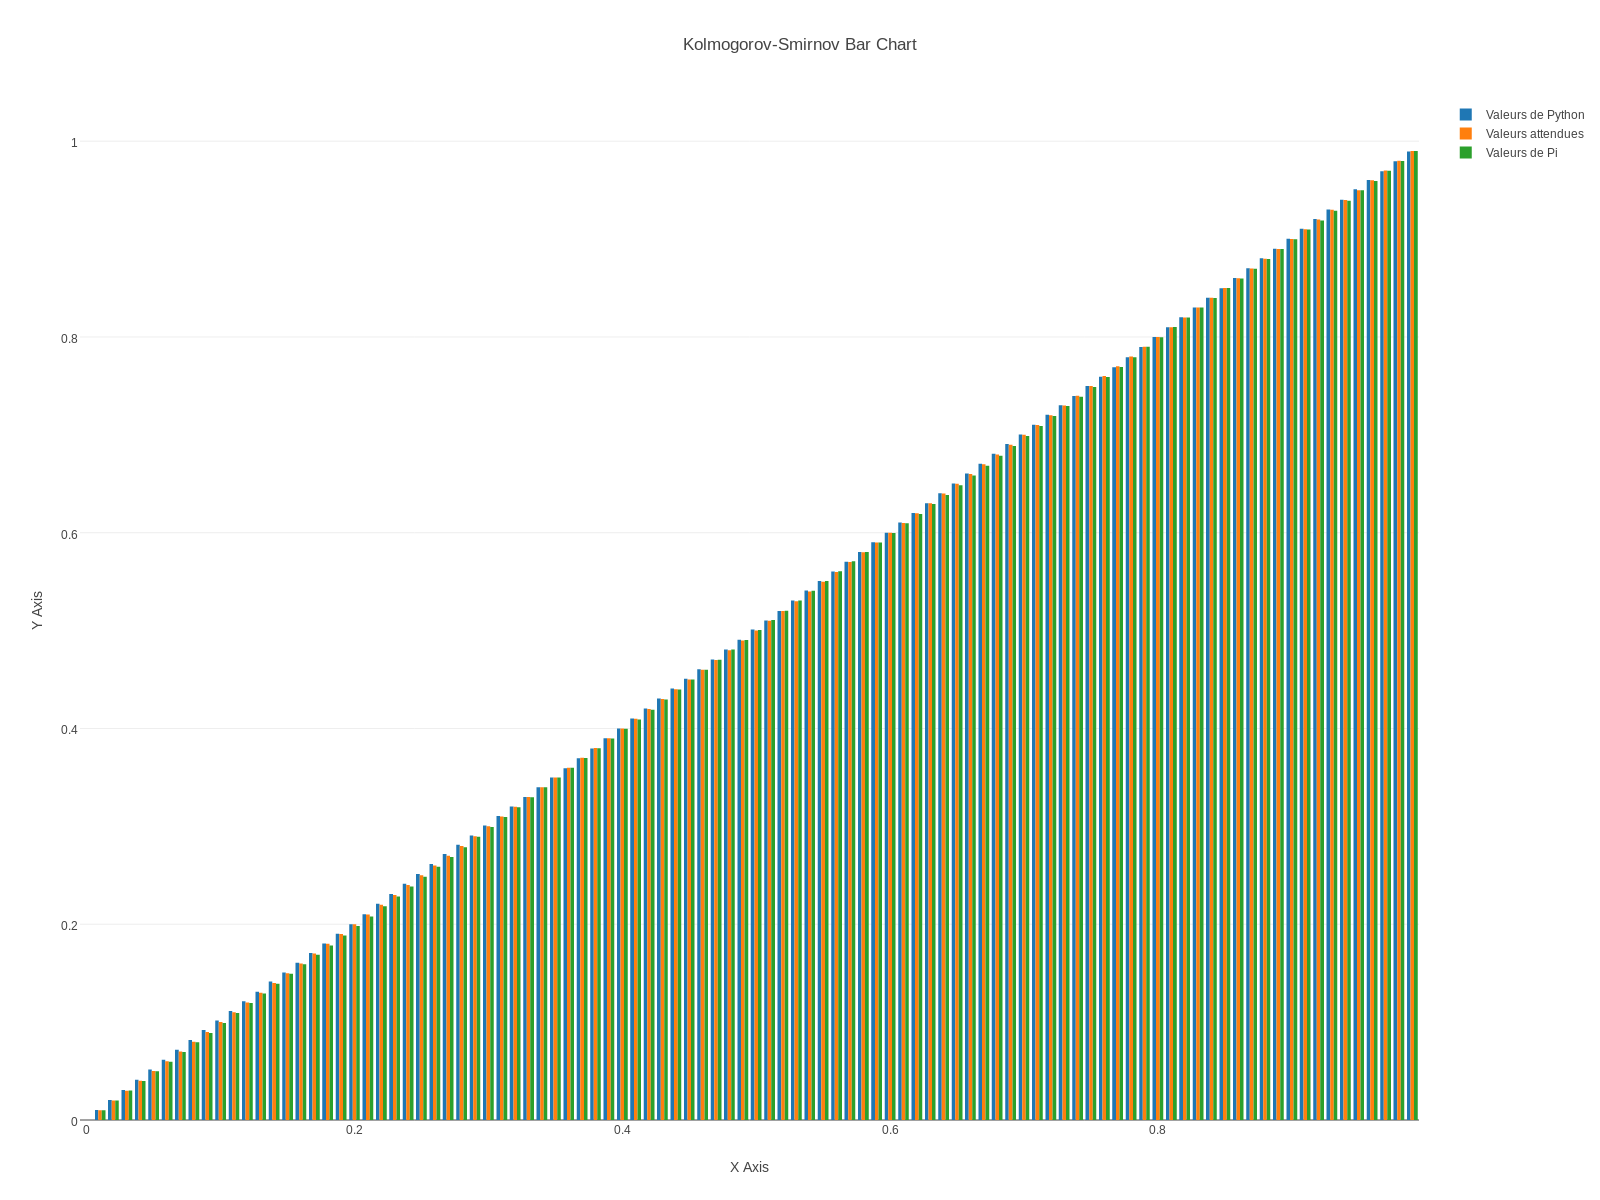
\includegraphics[scale=0.25]{../chart_images/kolmogorov-smirnov_bar_chart.png}
		\caption{Graphique de Kolmogorov-Smirnov}
	\end{figure}
	
	Écarts et valeurs critiques :
	\begin{figure}[h]
		\centering
		\begin{tabular}{|r|r|r|r|r|}
			\hline
			$\alpha$ & $D_n$ Pi & $D_n$ Python & $D_{\alpha}$ & Meilleur\\
			\hline
			0.001 & 0.000708 & 0.000849 & 0.001949 & Pi\\
			0.010 & 0.000708 & 0.000849 & 0.001628 & Pi\\
			0.050 & 0.000708 & 0.000849 & 0.001358 & Pi\\
			0.100 & 0.000708 & 0.000849 & 0.001224 & Pi\\
			\hline
		\end{tabular}
		\caption{Tableau de Kolmogorov-Smirnov}
	\end{figure}
	
	Nous remarquons que les deux générateurs passent ce test avec tous les $\alpha$ choisis.
	Nous remarquons également que notre générateur fait mieux que le générateur de Python.
	
	Attention cependant à l'interprétation hâtive des résultats.
	En effet, tant que nous n'avons pas étudié \textbf{tous} les nombres générés par les deux générateurs (l'entièreté de leur période), de nouveaux nombres pourraient apparaître lors d'une prochaine exécution. Nous pourrions donc obtenir un résultat différent.
	
	% TODO pourquoi pas tous les nombres ?
	
\newpage
\subsection{Test du gap}
Le test du gap est un test vérifiant la grandeur des trous (gap en anglais) séparant des nombres faisant partie d'un même intervalle.

Ce test se fait en différentes étapes:
\begin{itemize}
\item Nous générons n nombres à travers nos générateurs de nombres aléatoires.
\item Nous choisissons un intervalle $[a,b]\in[0,1]$ (nous avons ici choisis a=0 et b =1/2 pour un temps de calcul optimal).
\item Nous marquons les nombres se trouvant dans cet intervalle
\item Nous calculons les distances entre chaque nombres marqués (nous notons $r_i$ les différentes distances. 
\end{itemize} 

Nous obtenons ainsi les différentes occurrences $r_i$ que nous appelons les gaps (trous en anglais), et pouvons les comparer à l'aide d'un $\chi^2$ avec les valeurs théoriques attendues :

\[
	r_i = N p (1-p)^i
\] 
\[
	r_{>i} = N (1-p)^{i+1}
\]

où N est le nombres total de gaps observés

p est la probabilité d'être dans l'intervalle $[a,b]$ et vaut $b-a$


Nous avons donc effectuer ce test sur notre générateur pseudo-aléatoire et le générateur de python.

	\subsubsection{Notre générateur}

Ci-dessous nous avons illustrer les occurrences pour les différents gaps obtenus dans un tableau et à l'aide d'un graphique. 
Nous avons fixé la limite à 15 afin d'éviter les classes vides, ces dernières étant néfastes au test de $\chi^2$.

\begin{figure}[h]
	\centering
	\begin{tabular}{|r|r|r|}
		\hline
		APi Gap & Valeur attendue & Valeur observée\\
		\hline
		0 & 250101.000 & 250067\\
		1 & 125050.500 & 125248\\
		2 & 62525.250 & 62273\\
		3 & 31262.625 & 31471\\
		4 & 15631.312 & 15616\\
		5 & 7815.656 & 7860\\
		6 & 3907.828 & 3826\\
		7 & 1953.914 & 1898\\
		8 & 976.957 & 954\\
		9 & 488.479 & 471\\
		10 & 244.239 & 252\\
		11 & 122.120 & 135\\
		12 & 61.060 & 66\\
		13 & 30.530 & 30\\
		14 & 15.265 & 19\\
		> 15 & 15.265 & 16\\
		\hline
		Total & 500202 & 500202\\
		\hline
	\end{tabular}
	\caption{Tableau de Pi Gap}
\end{figure}

\begin{figure}[h]
\centering
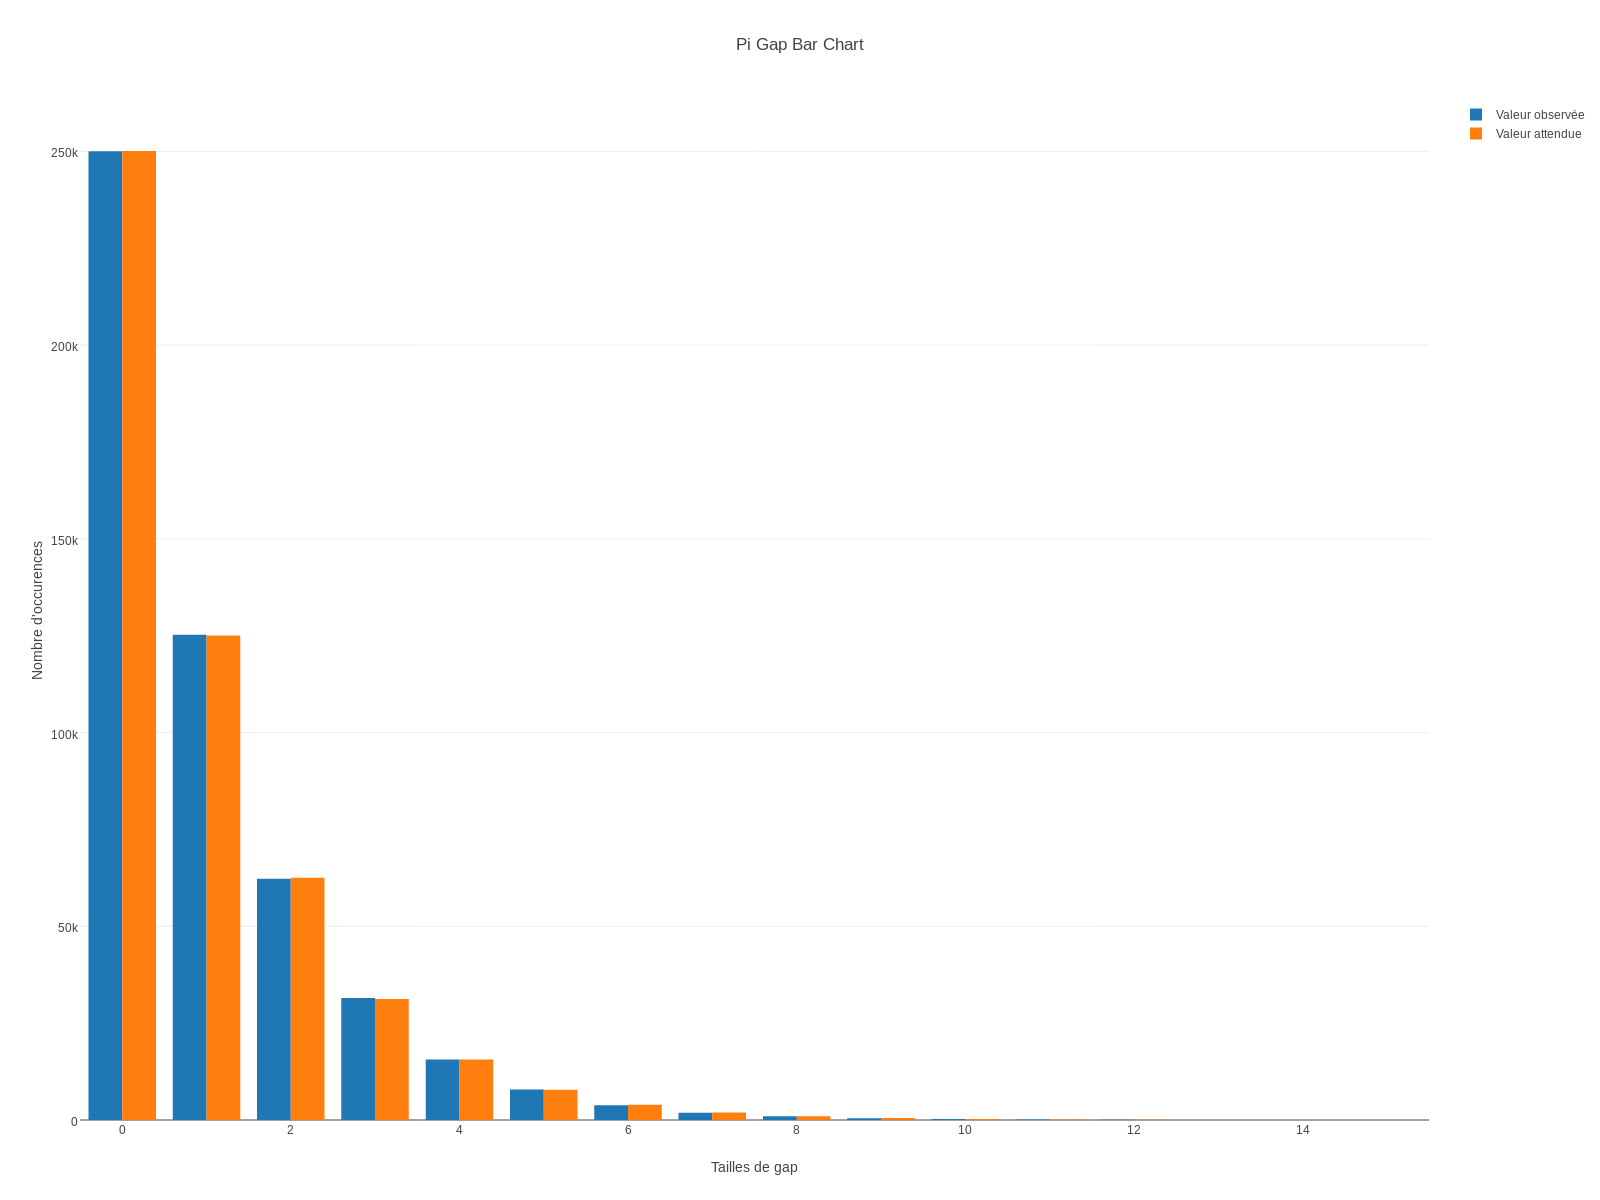
\includegraphics[scale=0.25]{../chart_images/pi_gap_bar_chart.png}
\caption{Graphique de Gap}
\end{figure}
\newpage

Résultats du test de $\chi^2$ :
\begin{figure}[h]
	\centering
	\begin{tabular}{|r|r|r|r|}
		\hline
		$\alpha$ & AValeur & Limite & Résultat\\
		\hline
		0.001 & 10.431 & 37.697 & réussi\\
		0.010 & 10.431 & 30.578 & réussi\\
		0.050 & 10.431 & 24.996 & réussi\\
		0.100 & 10.431 & 22.307 & réussi\\
		\hline
	\end{tabular}
	\caption{Tableau de $\chi^2$}
\end{figure}


Nous constatons donc que les différentes valeurs observées sont proches des valeurs théoriques. Et que le test de $\chi^2$ réussit bien. Notre générateur passe donc ce test avec succès.

\newpage

	\subsubsection{Le générateur de python}
En ce qui concerne ce générateur, nous avons procédé de la même façon que ci-dessus pour notre générateur.
	
\begin{figure}[h]
	\centering
	\begin{tabular}{|r|r|r|}
		\hline
		APython Gap & Valeur attendue & Valeur observée\\
		\hline
		0 & 249672.000 & 249152\\
		1 & 124836.000 & 125037\\
		2 & 62418.000 & 62606\\
		3 & 31209.000 & 31237\\
		4 & 15604.500 & 15686\\
		5 & 7802.250 & 7839\\
		6 & 3901.125 & 3834\\
		7 & 1950.562 & 1969\\
		8 & 975.281 & 942\\
		9 & 487.641 & 522\\
		10 & 243.820 & 254\\
		11 & 121.910 & 122\\
		12 & 60.955 & 78\\
		13 & 30.478 & 31\\
		14 & 15.239 & 19\\
		> 15 & 15.239 & 16\\
		\hline
		Total & 499344 & 499344\\
		\hline
	\end{tabular}
	\caption{Tableau de Python Gap}
\end{figure}

\newpage

\begin{figure}[h]
\centering
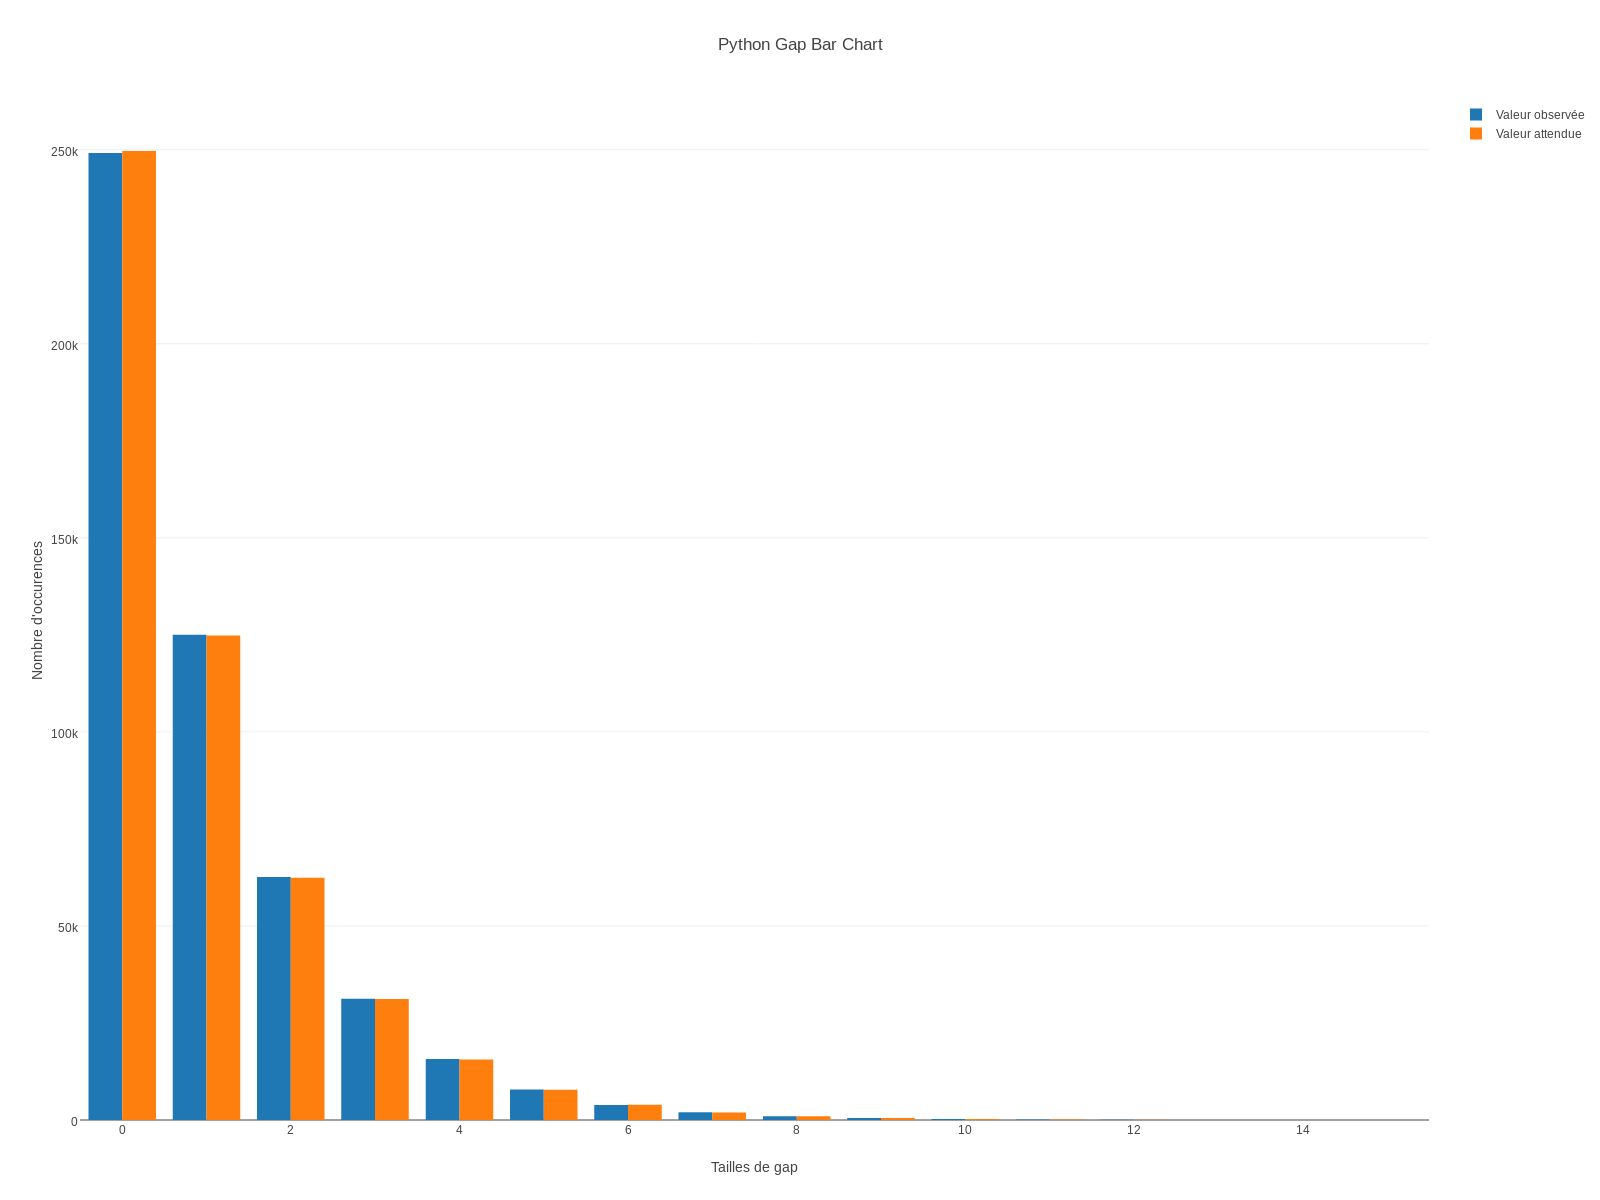
\includegraphics[scale=0.25]{../chart_images/python_gap_bar_chart.png}
\caption{Graphique de Gap}
\end{figure}

\begin{figure}[h]
	\centering
	\begin{tabular}{|r|r|r|r|}
		\hline
		$\alpha$ & AValeur & Limite & Résultat\\
		\hline
		0.001 & 13.649 & 37.697 & réussi\\
		0.010 & 13.649 & 30.578 & réussi\\
		0.050 & 13.649 & 24.996 & réussi\\
		0.100 & 13.649 & 22.307 & réussi\\
		\hline
	\end{tabular}
	\caption{Tableau de $\chi^2$}
\end{figure}


Nous observons, ici aussi, que les valeurs sont proches des valeurs théoriques et que le test de $\chi^2$  est réussi.

\subsubsection{Comparaison}

Les deux générateurs suivent une loi uniforme selon la réussite de ce test. 
Nous observons aussi que notre générateur réussit mieux ce test que celui de python.

\newpage

\subsection{Test du collectionneur de coupons}

Tout comme nous l'avons précédemment effectué sur les décimales de Pi, nous allons ici effectuer le même test sur le générateur de python et notre générateur. Nous avons ainsi pu comparer leurs résultats vis-à-vis de ce test.\\

Afin d'effectuer ce test comme précédemment, nous avons du avoir recourt à une petite adaptation. 

Nous avons donc discrétiser 1 million de nombres générés aléatoirement par python entre 0 et 1. Nous avons aussi utilisé la même méthode sur notre générateur. \\

Nous obtenons donc les tableaux de valeurs, les graphiques associés et les tests de $\chi^2$ suivants :

\begin{figure}[h]
\centering
\begin{tabular}{|r|r|r|}
\hline
tailles de séquences & Valeur attendue & Valeur observée\\
\hline
10 & 12.42718848 & 8\\
11 & 55.92234816 & 63\\
12 & 143.534026944 & 162\\
13 & 276.815623392 & 301\\
14 & 446.759911294 & 478\\
15 & 638.152283793 & 633\\
16 & 834.218397608 & 862\\
17 & 1020.00405762 & 1058\\
18 & 1184.16470752 & 1195\\
19 & 1319.46165499 & 1279\\
20 & 1422.43417043 & 1420\\
21 & 1492.66473313 & 1481\\
22 & 1531.93029943 & 1526\\
23 & 1543.41120583 & 1577\\
24 & 1531.03817211 & 1521\\
25 & 1498.99946609 & 1533\\
26 & 1451.39800026 & 1442\\
27 & 1392.03360299 & 1335\\
28 & 1324.2818821 & 1339\\
29 & 1251.0429409 & 1286\\
30 & 1174.73751011 & 1165\\
\hline
\end{tabular}
\caption{Tableau de Test du CDC : Notre générateur 1}
\end{figure}

\newpage

\begin{figure}[h]
\centering
\begin{tabular}{|r|r|r|}
\hline
tailles de séquences  & Valeur attendue & Valeur observée\\
\hline
31 & 1097.33297423 & 1072\\
32 & 1020.38635139 & 1005\\
33 & 945.095135062 & 983\\
34 & 872.349931581 & 864\\
35 & 802.785090265 & 741\\
36 & 736.825144986 & 744\\
37 & 674.726003239 & 666\\
38 & 616.610554842 & 625\\
39 & 562.498832208 & 539\\
40 & 512.333119704 & 508\\
50 & 190.639787783 & 188\\
60 & 67.7887123695 & 80\\
70 & 23.7786468984 & 23\\
80 & 8.30639112096 & 13\\
81 & 7.47643257483 & 11\\
82 & 6.7293337844 & 10\\
83 & 6.0568359896 & 4\\
84 & 5.45150086454 & 8\\
85 & 44.1708179912 & 43\\
\hline
\end{tabular}
\caption{Tableau de Test du CDC : Notre générateur 2}
\end{figure}

\newpage

\begin{figure}[h]
\centering
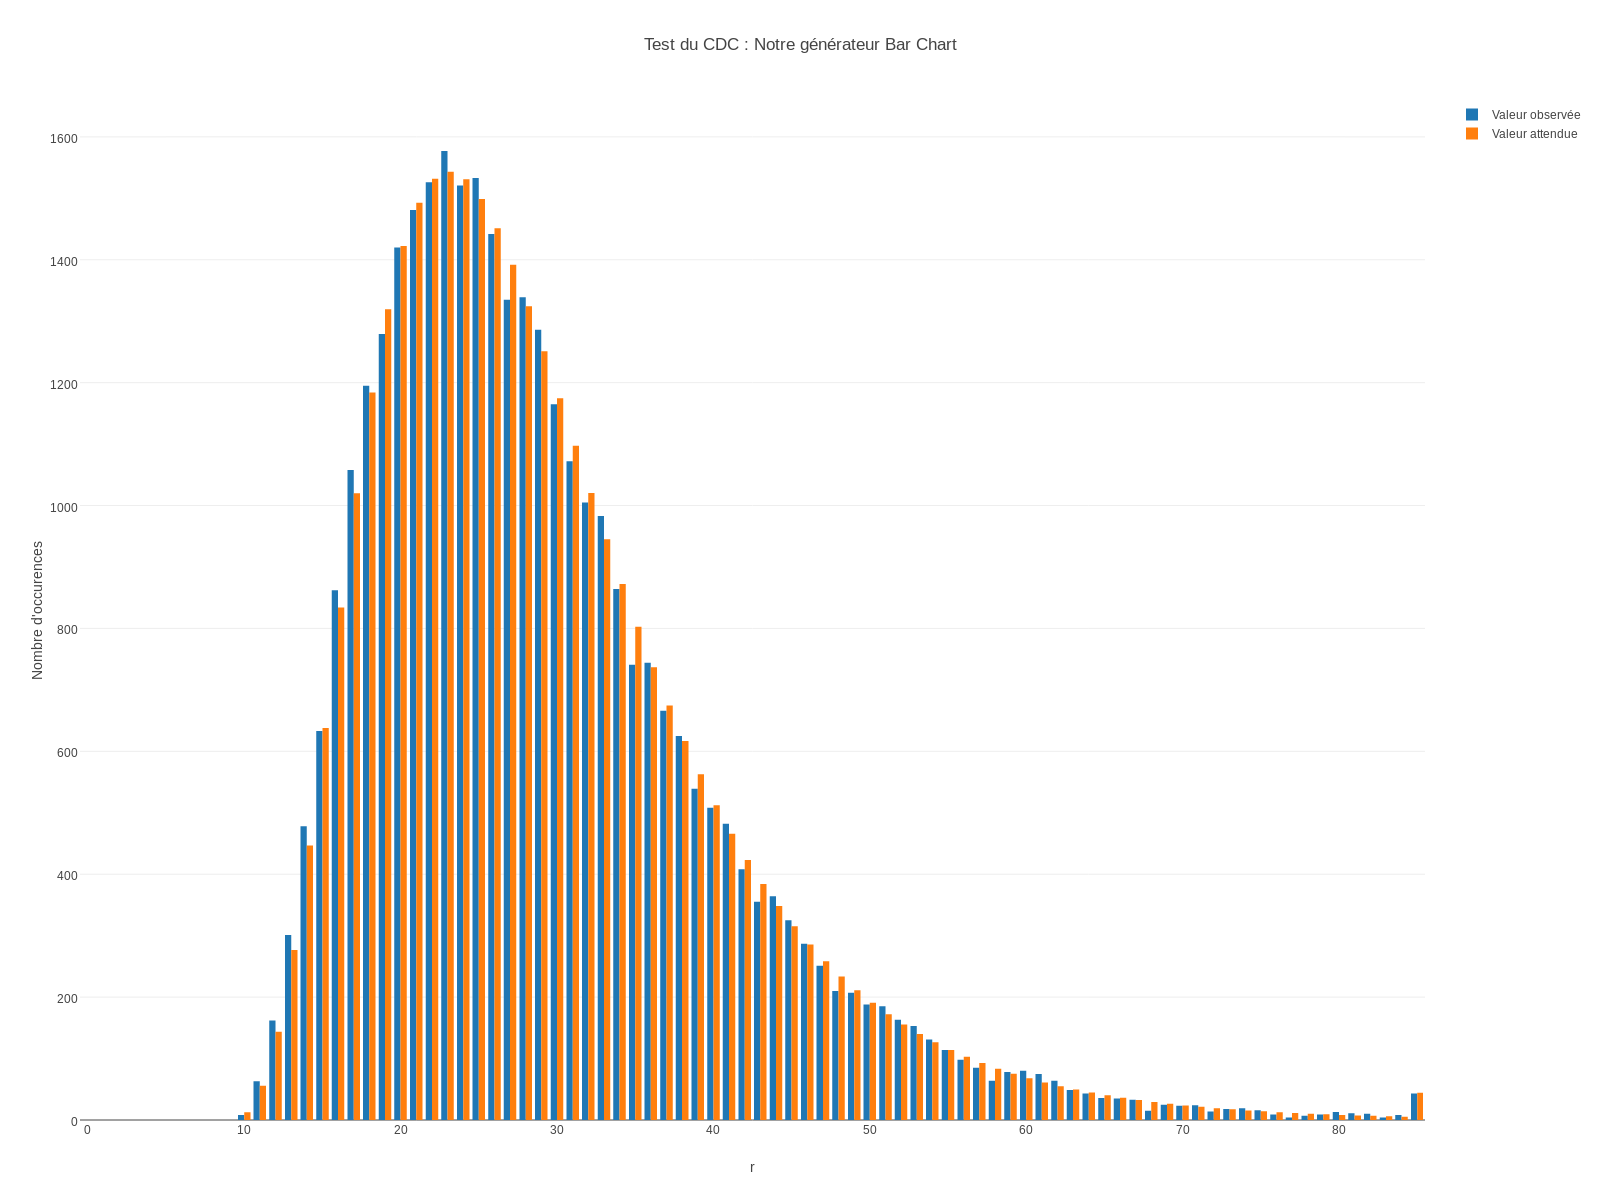
\includegraphics[scale=0.30]{../chart_images/cdc_ours.png}
\caption{Graphique de Test du CDC : Notre générateur}
\end{figure}

\begin{figure}[h]
\centering
\begin{tabular}{|r|r|r|r|}
\hline
$\alpha$ & AValeur & Limite & Résultat\\
\hline
0.001 & 73.868 & 131.041 & réussi\\
0.010 & 73.868 & 118.236 & réussi\\
0.050 & 73.868 & 107.522 & réussi\\
0.100 & 73.868 & 102.079 & réussi\\
\hline
\end{tabular}
\caption{Tableau de $\chi^2$}
\end{figure}

\newpage

\begin{figure}[h]
\centering
\begin{tabular}{|r|r|r|}
\hline
tailles de séquences & Valeur attendue & Valeur observée\\
\hline
10 & 12.4123104 & 14\\
11 & 55.8553968 & 50\\
12 & 143.36218512 & 143\\
13 & 276.48421416 & 308\\
14 & 446.225041342 & 448\\
15 & 637.388275044 & 664\\
16 & 833.219654563 & 835\\
17 & 1018.78288824 & 1041\\
18 & 1182.74700171 & 1200\\
19 & 1317.88196895 & 1306\\
20 & 1420.73120363 & 1363\\
21 & 1490.87768488 & 1487\\
22 & 1530.09624166 & 1510\\
23 & 1541.56340289 & 1505\\
24 & 1529.20518241 & 1511\\
25 & 1497.20483378 & 1489\\
26 & 1449.66035738 & 1468\\
27 & 1390.36703236 & 1349\\
28 & 1322.6964252 & 1356\\
29 & 1249.54516712 & 1258\\
30 & 1173.33109073 & 1213\\
31 & 1096.01922512 & 1121\\
32 & 1019.16472433 & 1030\\
33 & 943.963648157 & 986\\
34 & 871.305536697 & 840\\
35 & 801.823979808 & 799\\
36 & 735.943003103 & 718\\
37 & 673.918207697 & 693\\
38 & 615.872336284 & 610\\
39 & 561.825397292 & 545\\
40 & 511.719744189 & 513\\
50 & 190.411549995 & 192\\
60 & 67.7075543596 & 60\\
70 & 23.750178624 & 27\\
80 & 8.29644654244 & 7\\
81 & 7.46748163938 & 5\\
82 & 6.72127729064 & 5\\
83 & 6.04958462373 & 2\\
84 & 5.44497421806 & 5\\
85 & 44.1179357995 & 35\\
\hline
\end{tabular}
\caption{Tableau de Test du CDC : Le générateur de python }
\end{figure}
\newpage

\begin{figure}[h]
\centering
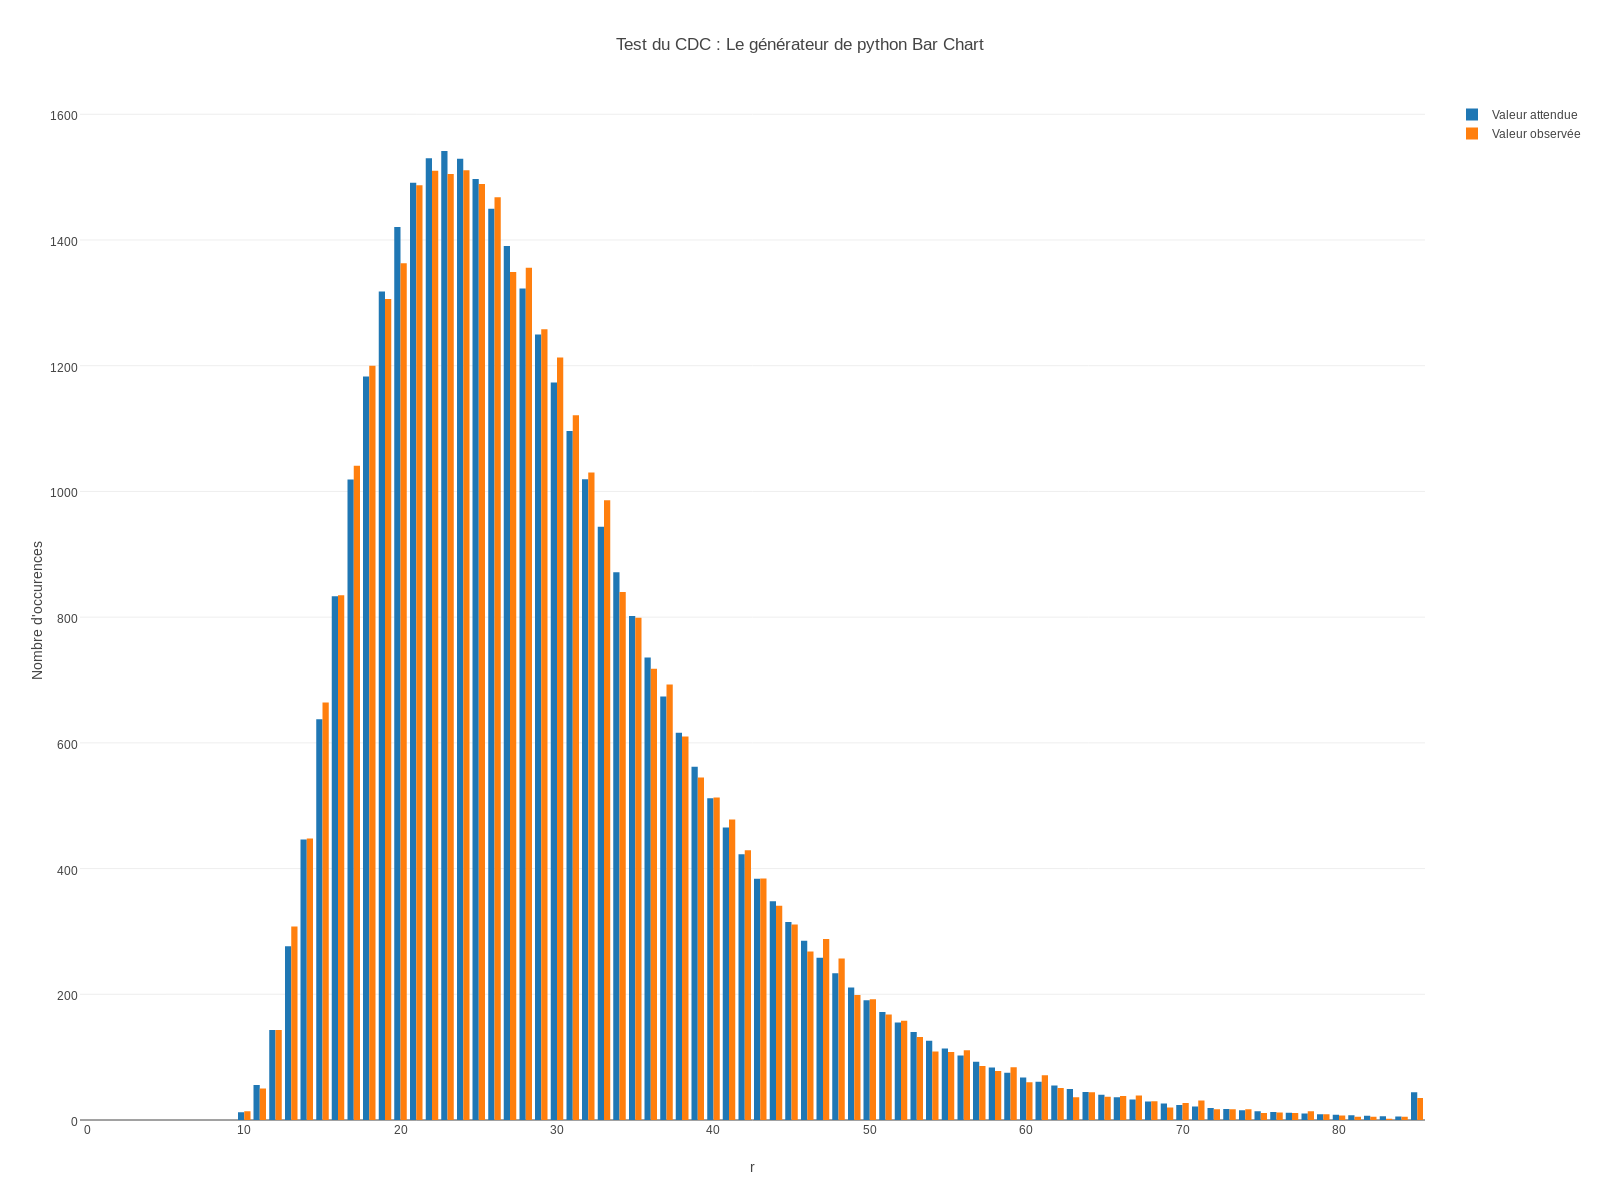
\includegraphics[scale=0.25]{../chart_images/cdc_py.png}
\caption{Graphique de Test du CDC : Le générateur de python}
\end{figure}

\begin{figure}[h]
\centering
\begin{tabular}{|r|r|r|r|}
\hline
$\alpha$ & AValeur & Limite & Résultat\\
\hline
0.001 & 56.083 & 131.041 & réussi\\
0.010 & 56.083 & 118.236 & réussi\\
0.050 & 56.083 & 107.522 & réussi\\
0.100 & 56.083 & 102.079 & réussi\\
\hline
\end{tabular}
\caption{Tableau de $\chi^2$}
\end{figure}
    
    
Nous pouvons donc conclure, par les tests réussis, que les 2 générateurs suivent la loi uniforme. Nous remarquons ici aussi que les valeurs respectent, dans les deux cas, la forme d'une gaussienne

Nous pouvons aussi constater que le générateur de python réussit mieux les tests que notre générateur basé sur les décimales de Pi. 
  	
	\newpage
	\subsection{Interprétation des résultats}
	Malgré la simplicité de notre générateur, celui-ci donne de très bons résultats.
	Cela peut s'expliquer par le fait que nous n'avons effectué nos tests que sur un nombre limité de nombres générés. 
	En effet, la période de notre générateur est de 200 000 alors que la période du générateur de Python (Mersenne Twister) est de $2^{19937}$.
	
	On constate aussi que sur certains tests, le générateur de python réussit mieux les tests que notre générateur. Sur d'autres, c'est l'inverse qui se produit.
	
	%TODO donner une conclusion sur les tests et pourquoi 
	
	On peut finalement conclure que les décimales de Pi, ainsi que nos deux générateurs suivent bien une loi uniforme d'après nos différents tests.	
	
	
	\section{Conclusion}
	Nous avons bien réalisé les objectifs fixés dans l'introduction, à savoir analyser le caractère aléatoire des décimales de pi, construire un générateur uniforme et le comparer au générateur par défaut de Python.
	
	Nous avons ainsi eu l'occasion de mettre en pratique et d'approfondir les concepts vus au cours théorique notamment les test de $\chi^2$, le test du poker, le test de Kolmogorov-Smirnov, le test de gap et le test du collectionneur de coupons.
	
	Nous tenons à remercier le titulaire BUYS Alain pour le dévouement dont il a fait preuve cette année.
	
\end{document}